% Created by tikzDevice version 0.12 on 2019-05-07 15:15:52
% !TEX encoding = UTF-8 Unicode
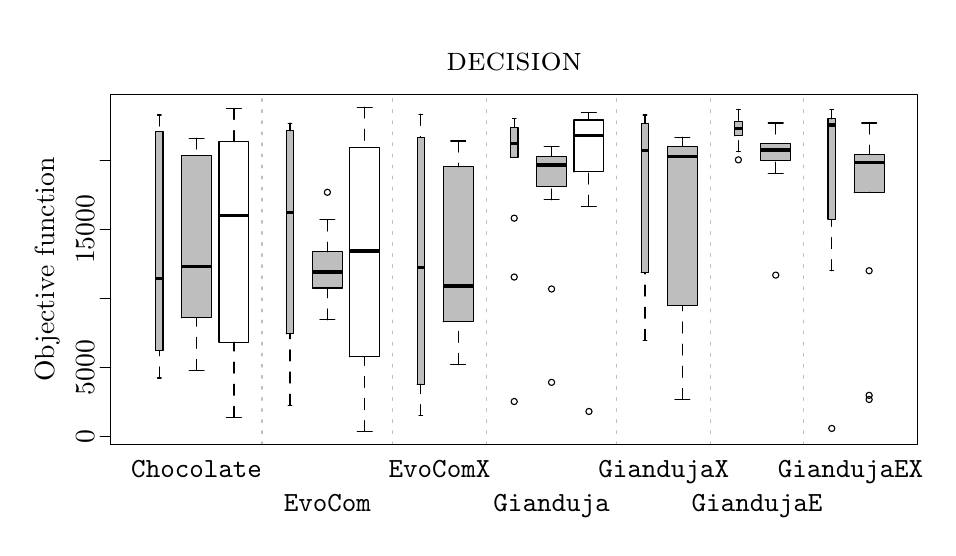
\begin{tikzpicture}[x=1pt,y=1pt]
\definecolor{fillColor}{RGB}{255,255,255}
\path[use as bounding box,fill=fillColor,fill opacity=0.00] (0,0) rectangle (325.21,180.67);
\begin{scope}
\path[clip] ( 30.00, 30.00) rectangle (321.61,156.67);
\definecolor{fillColor}{RGB}{190,190,190}

\path[fill=fillColor] ( 46.20, 64.00) --
	( 48.90, 64.00) --
	( 48.90,143.20) --
	( 46.20,143.20) --
	cycle;
\definecolor{drawColor}{RGB}{0,0,0}

\path[draw=drawColor,line width= 1.2pt,line join=round] ( 46.20, 90.01) -- ( 48.90, 90.01);

\path[draw=drawColor,line width= 0.4pt,dash pattern=on 4pt off 4pt ,line join=round,line cap=round] ( 47.55, 54.08) -- ( 47.55, 64.00);

\path[draw=drawColor,line width= 0.4pt,dash pattern=on 4pt off 4pt ,line join=round,line cap=round] ( 47.55,149.13) -- ( 47.55,143.20);

\path[draw=drawColor,line width= 0.4pt,line join=round,line cap=round] ( 46.88, 54.08) -- ( 48.23, 54.08);

\path[draw=drawColor,line width= 0.4pt,line join=round,line cap=round] ( 46.88,149.13) -- ( 48.23,149.13);

\path[draw=drawColor,line width= 0.4pt,line join=round,line cap=round] ( 46.20, 64.00) --
	( 48.90, 64.00) --
	( 48.90,143.20) --
	( 46.20,143.20) --
	( 46.20, 64.00);

\path[fill=fillColor] ( 55.65, 75.79) --
	( 66.45, 75.79) --
	( 66.45,134.63) --
	( 55.65,134.63) --
	cycle;

\path[draw=drawColor,line width= 1.2pt,line join=round] ( 55.65, 94.49) -- ( 66.45, 94.49);

\path[draw=drawColor,line width= 0.4pt,dash pattern=on 4pt off 4pt ,line join=round,line cap=round] ( 61.05, 56.79) -- ( 61.05, 75.79);

\path[draw=drawColor,line width= 0.4pt,dash pattern=on 4pt off 4pt ,line join=round,line cap=round] ( 61.05,140.78) -- ( 61.05,134.63);

\path[draw=drawColor,line width= 0.4pt,line join=round,line cap=round] ( 58.35, 56.79) -- ( 63.75, 56.79);

\path[draw=drawColor,line width= 0.4pt,line join=round,line cap=round] ( 58.35,140.78) -- ( 63.75,140.78);

\path[draw=drawColor,line width= 0.4pt,line join=round,line cap=round] ( 55.65, 75.79) --
	( 66.45, 75.79) --
	( 66.45,134.63) --
	( 55.65,134.63) --
	( 55.65, 75.79);
\definecolor{fillColor}{RGB}{255,255,255}

\path[fill=fillColor] ( 69.15, 66.99) --
	( 79.95, 66.99) --
	( 79.95,139.48) --
	( 69.15,139.48) --
	cycle;

\path[draw=drawColor,line width= 1.2pt,line join=round] ( 69.15,112.85) -- ( 79.95,112.85);

\path[draw=drawColor,line width= 0.4pt,dash pattern=on 4pt off 4pt ,line join=round,line cap=round] ( 74.55, 39.82) -- ( 74.55, 66.99);

\path[draw=drawColor,line width= 0.4pt,dash pattern=on 4pt off 4pt ,line join=round,line cap=round] ( 74.55,151.50) -- ( 74.55,139.48);

\path[draw=drawColor,line width= 0.4pt,line join=round,line cap=round] ( 71.85, 39.82) -- ( 77.25, 39.82);

\path[draw=drawColor,line width= 0.4pt,line join=round,line cap=round] ( 71.85,151.50) -- ( 77.25,151.50);

\path[draw=drawColor,line width= 0.4pt,line join=round,line cap=round] ( 69.15, 66.99) --
	( 79.95, 66.99) --
	( 79.95,139.48) --
	( 69.15,139.48) --
	( 69.15, 66.99);
\definecolor{fillColor}{RGB}{190,190,190}

\path[fill=fillColor] ( 93.45, 70.05) --
	( 96.15, 70.05) --
	( 96.15,143.45) --
	( 93.45,143.45) --
	cycle;

\path[draw=drawColor,line width= 1.2pt,line join=round] ( 93.45,113.98) -- ( 96.15,113.98);

\path[draw=drawColor,line width= 0.4pt,dash pattern=on 4pt off 4pt ,line join=round,line cap=round] ( 94.80, 44.24) -- ( 94.80, 70.05);

\path[draw=drawColor,line width= 0.4pt,dash pattern=on 4pt off 4pt ,line join=round,line cap=round] ( 94.80,146.18) -- ( 94.80,143.45);

\path[draw=drawColor,line width= 0.4pt,line join=round,line cap=round] ( 94.13, 44.24) -- ( 95.48, 44.24);

\path[draw=drawColor,line width= 0.4pt,line join=round,line cap=round] ( 94.13,146.18) -- ( 95.48,146.18);

\path[draw=drawColor,line width= 0.4pt,line join=round,line cap=round] ( 93.45, 70.05) --
	( 96.15, 70.05) --
	( 96.15,143.45) --
	( 93.45,143.45) --
	( 93.45, 70.05);

\path[fill=fillColor] (102.90, 86.60) --
	(113.70, 86.60) --
	(113.70, 99.67) --
	(102.90, 99.67) --
	cycle;

\path[draw=drawColor,line width= 1.2pt,line join=round] (102.90, 92.41) -- (113.70, 92.41);

\path[draw=drawColor,line width= 0.4pt,dash pattern=on 4pt off 4pt ,line join=round,line cap=round] (108.30, 75.08) -- (108.30, 86.60);

\path[draw=drawColor,line width= 0.4pt,dash pattern=on 4pt off 4pt ,line join=round,line cap=round] (108.30,111.20) -- (108.30, 99.67);

\path[draw=drawColor,line width= 0.4pt,line join=round,line cap=round] (105.60, 75.08) -- (111.00, 75.08);

\path[draw=drawColor,line width= 0.4pt,line join=round,line cap=round] (105.60,111.20) -- (111.00,111.20);

\path[draw=drawColor,line width= 0.4pt,line join=round,line cap=round] (102.90, 86.60) --
	(113.70, 86.60) --
	(113.70, 99.67) --
	(102.90, 99.67) --
	(102.90, 86.60);

\path[draw=drawColor,line width= 0.4pt,line join=round,line cap=round] (108.30,121.18) circle (  1.12);
\definecolor{fillColor}{RGB}{255,255,255}

\path[fill=fillColor] (116.40, 61.71) --
	(127.20, 61.71) --
	(127.20,137.32) --
	(116.40,137.32) --
	cycle;

\path[draw=drawColor,line width= 1.2pt,line join=round] (116.40, 99.93) -- (127.20, 99.93);

\path[draw=drawColor,line width= 0.4pt,dash pattern=on 4pt off 4pt ,line join=round,line cap=round] (121.80, 34.69) -- (121.80, 61.71);

\path[draw=drawColor,line width= 0.4pt,dash pattern=on 4pt off 4pt ,line join=round,line cap=round] (121.80,151.98) -- (121.80,137.32);

\path[draw=drawColor,line width= 0.4pt,line join=round,line cap=round] (119.10, 34.69) -- (124.50, 34.69);

\path[draw=drawColor,line width= 0.4pt,line join=round,line cap=round] (119.10,151.98) -- (124.50,151.98);

\path[draw=drawColor,line width= 0.4pt,line join=round,line cap=round] (116.40, 61.71) --
	(127.20, 61.71) --
	(127.20,137.32) --
	(116.40,137.32) --
	(116.40, 61.71);
\definecolor{fillColor}{RGB}{190,190,190}

\path[fill=fillColor] (140.71, 51.87) --
	(143.41, 51.87) --
	(143.41,141.12) --
	(140.71,141.12) --
	cycle;

\path[draw=drawColor,line width= 1.2pt,line join=round] (140.71, 94.06) -- (143.41, 94.06);

\path[draw=drawColor,line width= 0.4pt,dash pattern=on 4pt off 4pt ,line join=round,line cap=round] (142.06, 40.46) -- (142.06, 51.87);

\path[draw=drawColor,line width= 0.4pt,dash pattern=on 4pt off 4pt ,line join=round,line cap=round] (142.06,149.38) -- (142.06,141.12);

\path[draw=drawColor,line width= 0.4pt,line join=round,line cap=round] (141.38, 40.46) -- (142.73, 40.46);

\path[draw=drawColor,line width= 0.4pt,line join=round,line cap=round] (141.38,149.38) -- (142.73,149.38);

\path[draw=drawColor,line width= 0.4pt,line join=round,line cap=round] (140.71, 51.87) --
	(143.41, 51.87) --
	(143.41,141.12) --
	(140.71,141.12) --
	(140.71, 51.87);

\path[fill=fillColor] (150.16, 74.35) --
	(160.96, 74.35) --
	(160.96,130.35) --
	(150.16,130.35) --
	cycle;

\path[draw=drawColor,line width= 1.2pt,line join=round] (150.16, 87.33) -- (160.96, 87.33);

\path[draw=drawColor,line width= 0.4pt,dash pattern=on 4pt off 4pt ,line join=round,line cap=round] (155.56, 58.94) -- (155.56, 74.35);

\path[draw=drawColor,line width= 0.4pt,dash pattern=on 4pt off 4pt ,line join=round,line cap=round] (155.56,139.73) -- (155.56,130.35);

\path[draw=drawColor,line width= 0.4pt,line join=round,line cap=round] (152.86, 58.94) -- (158.26, 58.94);

\path[draw=drawColor,line width= 0.4pt,line join=round,line cap=round] (152.86,139.73) -- (158.26,139.73);

\path[draw=drawColor,line width= 0.4pt,line join=round,line cap=round] (150.16, 74.35) --
	(160.96, 74.35) --
	(160.96,130.35) --
	(150.16,130.35) --
	(150.16, 74.35);

\path[fill=fillColor] (174.46,133.87) --
	(177.16,133.87) --
	(177.16,144.71) --
	(174.46,144.71) --
	cycle;

\path[draw=drawColor,line width= 1.2pt,line join=round] (174.46,138.76) -- (177.16,138.76);

\path[draw=drawColor,line width= 0.4pt,dash pattern=on 4pt off 4pt ,line join=round,line cap=round] (175.81,133.87) -- (175.81,133.87);

\path[draw=drawColor,line width= 0.4pt,dash pattern=on 4pt off 4pt ,line join=round,line cap=round] (175.81,147.74) -- (175.81,144.71);

\path[draw=drawColor,line width= 0.4pt,line join=round,line cap=round] (175.13,133.87) -- (176.48,133.87);

\path[draw=drawColor,line width= 0.4pt,line join=round,line cap=round] (175.13,147.74) -- (176.48,147.74);

\path[draw=drawColor,line width= 0.4pt,line join=round,line cap=round] (174.46,133.87) --
	(177.16,133.87) --
	(177.16,144.71) --
	(174.46,144.71) --
	(174.46,133.87);

\path[draw=drawColor,line width= 0.4pt,line join=round,line cap=round] (175.81, 90.56) circle (  1.12);

\path[draw=drawColor,line width= 0.4pt,line join=round,line cap=round] (175.81, 45.58) circle (  1.12);

\path[draw=drawColor,line width= 0.4pt,line join=round,line cap=round] (175.81,111.83) circle (  1.12);

\path[fill=fillColor] (183.91,123.23) --
	(194.71,123.23) --
	(194.71,134.23) --
	(183.91,134.23) --
	cycle;

\path[draw=drawColor,line width= 1.2pt,line join=round] (183.91,131.08) -- (194.71,131.08);

\path[draw=drawColor,line width= 0.4pt,dash pattern=on 4pt off 4pt ,line join=round,line cap=round] (189.31,118.44) -- (189.31,123.23);

\path[draw=drawColor,line width= 0.4pt,dash pattern=on 4pt off 4pt ,line join=round,line cap=round] (189.31,137.80) -- (189.31,134.23);

\path[draw=drawColor,line width= 0.4pt,line join=round,line cap=round] (186.61,118.44) -- (192.01,118.44);

\path[draw=drawColor,line width= 0.4pt,line join=round,line cap=round] (186.61,137.80) -- (192.01,137.80);

\path[draw=drawColor,line width= 0.4pt,line join=round,line cap=round] (183.91,123.23) --
	(194.71,123.23) --
	(194.71,134.23) --
	(183.91,134.23) --
	(183.91,123.23);

\path[draw=drawColor,line width= 0.4pt,line join=round,line cap=round] (189.31, 86.24) circle (  1.12);

\path[draw=drawColor,line width= 0.4pt,line join=round,line cap=round] (189.31, 52.50) circle (  1.12);
\definecolor{fillColor}{RGB}{255,255,255}

\path[fill=fillColor] (197.41,128.56) --
	(208.21,128.56) --
	(208.21,147.30) --
	(197.41,147.30) --
	cycle;

\path[draw=drawColor,line width= 1.2pt,line join=round] (197.41,141.76) -- (208.21,141.76);

\path[draw=drawColor,line width= 0.4pt,dash pattern=on 4pt off 4pt ,line join=round,line cap=round] (202.81,116.14) -- (202.81,128.56);

\path[draw=drawColor,line width= 0.4pt,dash pattern=on 4pt off 4pt ,line join=round,line cap=round] (202.81,149.89) -- (202.81,147.30);

\path[draw=drawColor,line width= 0.4pt,line join=round,line cap=round] (200.11,116.14) -- (205.51,116.14);

\path[draw=drawColor,line width= 0.4pt,line join=round,line cap=round] (200.11,149.89) -- (205.51,149.89);

\path[draw=drawColor,line width= 0.4pt,line join=round,line cap=round] (197.41,128.56) --
	(208.21,128.56) --
	(208.21,147.30) --
	(197.41,147.30) --
	(197.41,128.56);

\path[draw=drawColor,line width= 0.4pt,line join=round,line cap=round] (202.81, 41.98) circle (  1.12);
\definecolor{fillColor}{RGB}{190,190,190}

\path[fill=fillColor] (221.71, 92.16) --
	(224.41, 92.16) --
	(224.41,146.12) --
	(221.71,146.12) --
	cycle;

\path[draw=drawColor,line width= 1.2pt,line join=round] (221.71,136.24) -- (224.41,136.24);

\path[draw=drawColor,line width= 0.4pt,dash pattern=on 4pt off 4pt ,line join=round,line cap=round] (223.06, 67.67) -- (223.06, 92.16);

\path[draw=drawColor,line width= 0.4pt,dash pattern=on 4pt off 4pt ,line join=round,line cap=round] (223.06,149.13) -- (223.06,146.12);

\path[draw=drawColor,line width= 0.4pt,line join=round,line cap=round] (222.38, 67.67) -- (223.73, 67.67);

\path[draw=drawColor,line width= 0.4pt,line join=round,line cap=round] (222.38,149.13) -- (223.73,149.13);

\path[draw=drawColor,line width= 0.4pt,line join=round,line cap=round] (221.71, 92.16) --
	(224.41, 92.16) --
	(224.41,146.12) --
	(221.71,146.12) --
	(221.71, 92.16);

\path[fill=fillColor] (231.16, 80.22) --
	(241.96, 80.22) --
	(241.96,137.78) --
	(231.16,137.78) --
	cycle;

\path[draw=drawColor,line width= 1.2pt,line join=round] (231.16,134.12) -- (241.96,134.12);

\path[draw=drawColor,line width= 0.4pt,dash pattern=on 4pt off 4pt ,line join=round,line cap=round] (236.56, 46.32) -- (236.56, 80.22);

\path[draw=drawColor,line width= 0.4pt,dash pattern=on 4pt off 4pt ,line join=round,line cap=round] (236.56,141.13) -- (236.56,137.78);

\path[draw=drawColor,line width= 0.4pt,line join=round,line cap=round] (233.86, 46.32) -- (239.26, 46.32);

\path[draw=drawColor,line width= 0.4pt,line join=round,line cap=round] (233.86,141.13) -- (239.26,141.13);

\path[draw=drawColor,line width= 0.4pt,line join=round,line cap=round] (231.16, 80.22) --
	(241.96, 80.22) --
	(241.96,137.78) --
	(231.16,137.78) --
	(231.16, 80.22);

\path[fill=fillColor] (255.46,141.60) --
	(258.16,141.60) --
	(258.16,146.74) --
	(255.46,146.74) --
	cycle;

\path[draw=drawColor,line width= 1.2pt,line join=round] (255.46,144.33) -- (258.16,144.33);

\path[draw=drawColor,line width= 0.4pt,dash pattern=on 4pt off 4pt ,line join=round,line cap=round] (256.81,135.84) -- (256.81,141.60);

\path[draw=drawColor,line width= 0.4pt,dash pattern=on 4pt off 4pt ,line join=round,line cap=round] (256.81,151.14) -- (256.81,146.74);

\path[draw=drawColor,line width= 0.4pt,line join=round,line cap=round] (256.14,135.84) -- (257.49,135.84);

\path[draw=drawColor,line width= 0.4pt,line join=round,line cap=round] (256.14,151.14) -- (257.49,151.14);

\path[draw=drawColor,line width= 0.4pt,line join=round,line cap=round] (255.46,141.60) --
	(258.16,141.60) --
	(258.16,146.74) --
	(255.46,146.74) --
	(255.46,141.60);

\path[draw=drawColor,line width= 0.4pt,line join=round,line cap=round] (256.81,132.91) circle (  1.12);

\path[fill=fillColor] (264.91,132.72) --
	(275.71,132.72) --
	(275.71,138.85) --
	(264.91,138.85) --
	cycle;

\path[draw=drawColor,line width= 1.2pt,line join=round] (264.91,136.42) -- (275.71,136.42);

\path[draw=drawColor,line width= 0.4pt,dash pattern=on 4pt off 4pt ,line join=round,line cap=round] (270.31,128.09) -- (270.31,132.72);

\path[draw=drawColor,line width= 0.4pt,dash pattern=on 4pt off 4pt ,line join=round,line cap=round] (270.31,146.23) -- (270.31,138.85);

\path[draw=drawColor,line width= 0.4pt,line join=round,line cap=round] (267.61,128.09) -- (273.01,128.09);

\path[draw=drawColor,line width= 0.4pt,line join=round,line cap=round] (267.61,146.23) -- (273.01,146.23);

\path[draw=drawColor,line width= 0.4pt,line join=round,line cap=round] (264.91,132.72) --
	(275.71,132.72) --
	(275.71,138.85) --
	(264.91,138.85) --
	(264.91,132.72);

\path[draw=drawColor,line width= 0.4pt,line join=round,line cap=round] (270.31, 91.25) circle (  1.12);

\path[fill=fillColor] (289.21,111.42) --
	(291.91,111.42) --
	(291.91,147.74) --
	(289.21,147.74) --
	cycle;

\path[draw=drawColor,line width= 1.2pt,line join=round] (289.21,145.50) -- (291.91,145.50);

\path[draw=drawColor,line width= 0.4pt,dash pattern=on 4pt off 4pt ,line join=round,line cap=round] (290.56, 92.84) -- (290.56,111.42);

\path[draw=drawColor,line width= 0.4pt,dash pattern=on 4pt off 4pt ,line join=round,line cap=round] (290.56,151.14) -- (290.56,147.74);

\path[draw=drawColor,line width= 0.4pt,line join=round,line cap=round] (289.89, 92.84) -- (291.24, 92.84);

\path[draw=drawColor,line width= 0.4pt,line join=round,line cap=round] (289.89,151.14) -- (291.24,151.14);

\path[draw=drawColor,line width= 0.4pt,line join=round,line cap=round] (289.21,111.42) --
	(291.91,111.42) --
	(291.91,147.74) --
	(289.21,147.74) --
	(289.21,111.42);

\path[draw=drawColor,line width= 0.4pt,line join=round,line cap=round] (290.56, 35.86) circle (  1.12);

\path[fill=fillColor] (298.66,121.22) --
	(309.46,121.22) --
	(309.46,134.81) --
	(298.66,134.81) --
	cycle;

\path[draw=drawColor,line width= 1.2pt,line join=round] (298.66,131.96) -- (309.46,131.96);

\path[draw=drawColor,line width= 0.4pt,dash pattern=on 4pt off 4pt ,line join=round,line cap=round] (304.06,121.22) -- (304.06,121.22);

\path[draw=drawColor,line width= 0.4pt,dash pattern=on 4pt off 4pt ,line join=round,line cap=round] (304.06,146.23) -- (304.06,134.81);

\path[draw=drawColor,line width= 0.4pt,line join=round,line cap=round] (301.36,121.22) -- (306.76,121.22);

\path[draw=drawColor,line width= 0.4pt,line join=round,line cap=round] (301.36,146.23) -- (306.76,146.23);

\path[draw=drawColor,line width= 0.4pt,line join=round,line cap=round] (298.66,121.22) --
	(309.46,121.22) --
	(309.46,134.81) --
	(298.66,134.81) --
	(298.66,121.22);

\path[draw=drawColor,line width= 0.4pt,line join=round,line cap=round] (304.06, 92.84) circle (  1.12);

\path[draw=drawColor,line width= 0.4pt,line join=round,line cap=round] (304.06, 46.32) circle (  1.12);

\path[draw=drawColor,line width= 0.4pt,line join=round,line cap=round] (304.06, 47.81) circle (  1.12);
\definecolor{drawColor}{RGB}{190,190,190}

\path[draw=drawColor,line width= 0.4pt,dash pattern=on 1pt off 3pt ,line join=round,line cap=round] ( 84.68, 30.00) -- ( 84.68,156.67);

\path[draw=drawColor,line width= 0.4pt,dash pattern=on 1pt off 3pt ,line join=round,line cap=round] (131.93, 30.00) -- (131.93,156.67);

\path[draw=drawColor,line width= 0.4pt,dash pattern=on 1pt off 3pt ,line join=round,line cap=round] (165.68, 30.00) -- (165.68,156.67);

\path[draw=drawColor,line width= 0.4pt,dash pattern=on 1pt off 3pt ,line join=round,line cap=round] (212.93, 30.00) -- (212.93,156.67);

\path[draw=drawColor,line width= 0.4pt,dash pattern=on 1pt off 3pt ,line join=round,line cap=round] (246.69, 30.00) -- (246.69,156.67);

\path[draw=drawColor,line width= 0.4pt,dash pattern=on 1pt off 3pt ,line join=round,line cap=round] (280.44, 30.00) -- (280.44,156.67);
\end{scope}
\begin{scope}
\path[clip] (  0.00,  0.00) rectangle (325.21,180.67);
\definecolor{drawColor}{RGB}{0,0,0}

\node[text=drawColor,anchor=base,inner sep=0pt, outer sep=0pt, scale=  1.00] at ( 61.05, 18.00) {\texttt{Chocolate}};

\node[text=drawColor,anchor=base,inner sep=0pt, outer sep=0pt, scale=  1.00] at (148.81, 18.00) {\texttt{EvoComX}};

\node[text=drawColor,anchor=base,inner sep=0pt, outer sep=0pt, scale=  1.00] at (229.81, 18.00) {\texttt{GiandujaX}};

\node[text=drawColor,anchor=base,inner sep=0pt, outer sep=0pt, scale=  1.00] at (297.31, 18.00) {\texttt{GiandujaEX}};

\node[text=drawColor,anchor=base,inner sep=0pt, outer sep=0pt, scale=  1.00] at (108.30,  6.00) {\texttt{EvoCom}};

\node[text=drawColor,anchor=base,inner sep=0pt, outer sep=0pt, scale=  1.00] at (189.31,  6.00) {\texttt{Gianduja}};

\node[text=drawColor,anchor=base,inner sep=0pt, outer sep=0pt, scale=  1.00] at (263.56,  6.00) {\texttt{GiandujaE}};
\end{scope}
\begin{scope}
\path[clip] (  0.00,  0.00) rectangle (325.21,180.67);
\definecolor{drawColor}{RGB}{0,0,0}

\node[text=drawColor,anchor=base,inner sep=0pt, outer sep=0pt, scale=  1.20] at (175.81,165.07) {\textsc{decision}};

\node[text=drawColor,rotate= 90.00,anchor=base,inner sep=0pt, outer sep=0pt, scale=  1.00] at (  9.60, 93.34) {Objective function};
\end{scope}
\begin{scope}
\path[clip] (  0.00,  0.00) rectangle (325.21,180.67);
\definecolor{drawColor}{RGB}{0,0,0}

\path[draw=drawColor,line width= 0.4pt,line join=round,line cap=round] ( 30.00, 32.88) -- ( 30.00,132.81);

\path[draw=drawColor,line width= 0.4pt,line join=round,line cap=round] ( 30.00, 32.88) -- ( 26.20, 32.88);

\path[draw=drawColor,line width= 0.4pt,line join=round,line cap=round] ( 30.00, 57.86) -- ( 26.20, 57.86);

\path[draw=drawColor,line width= 0.4pt,line join=round,line cap=round] ( 30.00, 82.84) -- ( 26.20, 82.84);

\path[draw=drawColor,line width= 0.4pt,line join=round,line cap=round] ( 30.00,107.82) -- ( 26.20,107.82);

\path[draw=drawColor,line width= 0.4pt,line join=round,line cap=round] ( 30.00,132.81) -- ( 26.20,132.81);

\node[text=drawColor,rotate= 90.00,anchor=base,inner sep=0pt, outer sep=0pt, scale=  1.00] at ( 24.00, 32.88) {0};

\node[text=drawColor,rotate= 90.00,anchor=base,inner sep=0pt, outer sep=0pt, scale=  1.00] at ( 24.00, 57.86) {5000};

\node[text=drawColor,rotate= 90.00,anchor=base,inner sep=0pt, outer sep=0pt, scale=  1.00] at ( 24.00,107.82) {15000};

\path[draw=drawColor,line width= 0.4pt,line join=round,line cap=round] ( 30.00, 30.00) --
	(321.61, 30.00) --
	(321.61,156.67) --
	( 30.00,156.67) --
	( 30.00, 30.00);
\end{scope}
\end{tikzpicture}
